\chapter{Casos de uso}

%Los casos de uso se identificarán de acuerdo a la siguiente nomenclatura:

%- - - - - - - - - - - - - - - - - - - - - - - - - - - - -
\section{Especificación de casos de uso}

Para poder entender un caso de uso más allá de un diagrama, se lleva a cabo la tarea de especificar cada uno de los casos de uso identificados en el sistema con el fin de describir las secuencias de acciones que realiza el sistema y que lleva a un resultado de valor a un actor específico. Los casos de uso tienen atributos los cuales se describen a continuación:

\begin{description}
	\item[Id] Identificador del caso de uso, el cual debe ser único.
	\item[Nombre] Nombre del caso de uso el cual es descriptivo basándose en la transacción que se realiza.
	\item[Resumen] Es una descripción resumida en la que se especifica la transacción realizada por el caso de uso.
	\item[Actores] Lista de los actores que interactúan con el caso de uso.
	\item[Entradas] Lista los datos de entrada que el caso de uso recibe, los cuales harán referencia al modelo de información.
	\item[Salidas] Lista los datos de salida que el caso de uso genera.
	\item[Destino] Indica a dónde se dirigen los datos de salida, por ejemplo: interfaz, impresora, repositorio, hacia un servidor o un archivo.
	\item[Precondiciones] Enlista las cosas que deben haber sucedido para que el caso  de uso se lleve a cabo.
	\item[Postcondiciones] Enlista las cosas que suceden en el sistema o negocio de forma inmediata o a corto plazo una vez que se ejecute el caso de uso.
	\item[Reglas de Negocio] Lista las reglas de negocio que se van a ejecutar en el caso de uso.
	\item[Viene de] Indica cuando el caso de uso se extiende de otro o se incluye en otro.
	\item[Casos de prueba] Indican los datos o condiciones con las que se debe probar este caso de uso.
	\item[Trayectoria principal] Secuencia de pasos que llevan al caso de uso al éxito.
	\item[Trayectoria(s) alternativa(s)] Secuencias de pasos que llevan al caso de uso al éxito o al fracaso.
	\item[Puntos de extensión] Cuando existen casos de uso que pueden ejecutarse a partir del caso de uso en proceso.
\end{description}

\section{Módulo General}
	En la figura \ref{adcu:grl} se muestra el diagrama de casos de uso del módulo general del sistema.

	\begin{figure}[hbtp!]
		\begin{center}
			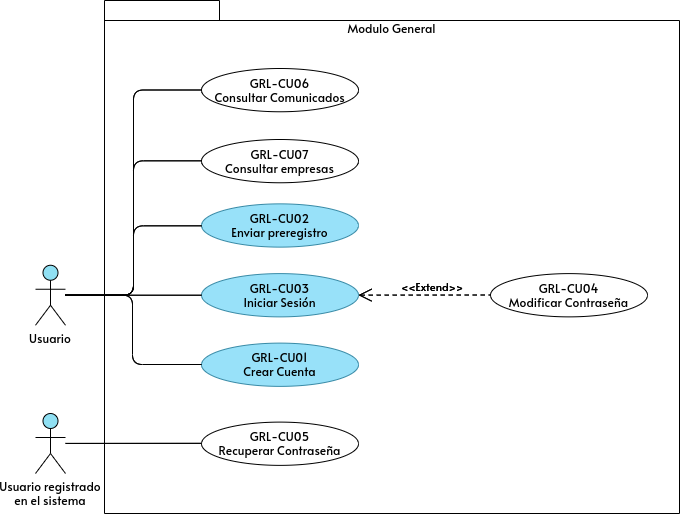
\includegraphics[width=.8\textwidth]{sprints/imagenes/CUGRL.png}
		\end{center}
		
		\caption{Diagrama de casos de uso del \textit{Módulo General}.}
		\label{adcu:grl}
	\end{figure}

	\begin{itemize}
        \item Los casos de uso \IUazul{} , son aquellos que se pertenecen a esta primera entrega del proyecto.
        \item Los casos de uso \IUblanco{}, se tienen planeados para la segunda entrega del proyecto.
    \end{itemize} 

	\begin{UseCase}[]{USR-CU03.3}{ELiminar Idioma}{
	%Permite al alumno consultar la información de sus idiomas registrados en el perfil.
}
	%----------------------------------------------------------------
	% Datos generales del CU:
	\UCsection{Atributos}
	\UCitem{Actor(es)}{
		\Titem Candidato. 
	}
	\UCitem[admin]{Prioridad}{ 
		\Titem Media.
	}
	\UCitem[admin]{Complejidad}{
		\Titem Baja
	}
	\UCitem{Precondiciones}{
		\Titem El alumno debe de tener una cuenta en el sistema.
		\Titem Se debe de tener previmante registrado al menos un idioma.
	}
	\UCitem{Destino}{
		\Titem \refElem{USR-IU03.1}
	}
	\UCitem{Reglas de Negocio}{
		\Titem Ninguna.
		
	}
	\UCitem{Viene de}{
		\Titem Caso de uso \refIdElem{USR-CU03}.
	}	
\end{UseCase}

%Trayectoria Principal
\begin{UCtrayectoria}
	\UCpaso [\UCactor] Presiona el botón \IUEliminar{} desde la interfaz \refElem{USR-IU03}.
    \UCpaso [\UCsist] Muestra la interfaz \refElem{USR-IU03.3}.
	\UCpaso [\UCactor] Presiona el botón \IUbutton{Aceptar}.\refTray{A}
	\UCpaso [\UCsist] Agrega al catalogo de idiomas el idioma que se quiere eliminar.
	\UCpaso [\UCsist] Eliminar el registro del idioma en el sistem.
	\UCpaso [\UCsist] Muestra la información actualizada en la interfaz \refElem{USR-IU03}.
\end{UCtrayectoria}

\begin{UCtrayectoriaA}[Fin del caso de uso]{A}{El actor desea cancelar el registro}
	\UCpaso [\UCsist] Presiona el botón \IUbutton{Cancelar}.
	\extendUC{USR-CU03}.
\end{UCtrayectoriaA} 


	\clearpage
\subsection{USR-IU02.2 Editar Medios de contacto y redes sociales}

\subsubsection{Objetivo}
En la figura \refElem{USR-IU02.2} se muestra la interfaz correspondiente con la funcionalidad descrita en las
trayectorias del caso de uso \refElem{USR-CU02.2} , la cual permite al actor editar sus medios de contacto como son: correos, teléfonos y redes sociales.

\subsubsection{Comandos}
Los siguientes comandos aparecen en la interfaz descrita anteriormente.
\Titem \IUbutton{Aceptar} : Cuando presiona el botón, actualiza la información .
\Titem \IUbutton{Cancelar} : Cuando presiona el botón, muestra la sección anterior.%\refElem{GRL-IU02-2}.

\IUfig{.9}{CasosdeUso/USR-CU02-2/imagenes/USR-IU02.2.png}{USR-IU02.2}{Editar Medios de contacto y redes sociales}  


\clearpage


	\begin{UseCase}[]{USR-CU03.3}{ELiminar Idioma}{
	%Permite al alumno consultar la información de sus idiomas registrados en el perfil.
}
	%----------------------------------------------------------------
	% Datos generales del CU:
	\UCsection{Atributos}
	\UCitem{Actor(es)}{
		\Titem Candidato. 
	}
	\UCitem[admin]{Prioridad}{ 
		\Titem Media.
	}
	\UCitem[admin]{Complejidad}{
		\Titem Baja
	}
	\UCitem{Precondiciones}{
		\Titem El alumno debe de tener una cuenta en el sistema.
		\Titem Se debe de tener previmante registrado al menos un idioma.
	}
	\UCitem{Destino}{
		\Titem \refElem{USR-IU03.1}
	}
	\UCitem{Reglas de Negocio}{
		\Titem Ninguna.
		
	}
	\UCitem{Viene de}{
		\Titem Caso de uso \refIdElem{USR-CU03}.
	}	
\end{UseCase}

%Trayectoria Principal
\begin{UCtrayectoria}
	\UCpaso [\UCactor] Presiona el botón \IUEliminar{} desde la interfaz \refElem{USR-IU03}.
    \UCpaso [\UCsist] Muestra la interfaz \refElem{USR-IU03.3}.
	\UCpaso [\UCactor] Presiona el botón \IUbutton{Aceptar}.\refTray{A}
	\UCpaso [\UCsist] Agrega al catalogo de idiomas el idioma que se quiere eliminar.
	\UCpaso [\UCsist] Eliminar el registro del idioma en el sistem.
	\UCpaso [\UCsist] Muestra la información actualizada en la interfaz \refElem{USR-IU03}.
\end{UCtrayectoria}

\begin{UCtrayectoriaA}[Fin del caso de uso]{A}{El actor desea cancelar el registro}
	\UCpaso [\UCsist] Presiona el botón \IUbutton{Cancelar}.
	\extendUC{USR-CU03}.
\end{UCtrayectoriaA} 


	\clearpage
\subsection{USR-IU02.2 Editar Medios de contacto y redes sociales}

\subsubsection{Objetivo}
En la figura \refElem{USR-IU02.2} se muestra la interfaz correspondiente con la funcionalidad descrita en las
trayectorias del caso de uso \refElem{USR-CU02.2} , la cual permite al actor editar sus medios de contacto como son: correos, teléfonos y redes sociales.

\subsubsection{Comandos}
Los siguientes comandos aparecen en la interfaz descrita anteriormente.
\Titem \IUbutton{Aceptar} : Cuando presiona el botón, actualiza la información .
\Titem \IUbutton{Cancelar} : Cuando presiona el botón, muestra la sección anterior.%\refElem{GRL-IU02-2}.

\IUfig{.9}{CasosdeUso/USR-CU02-2/imagenes/USR-IU02.2.png}{USR-IU02.2}{Editar Medios de contacto y redes sociales}  


\clearpage


	\begin{UseCase}[]{USR-CU03.3}{ELiminar Idioma}{
	%Permite al alumno consultar la información de sus idiomas registrados en el perfil.
}
	%----------------------------------------------------------------
	% Datos generales del CU:
	\UCsection{Atributos}
	\UCitem{Actor(es)}{
		\Titem Candidato. 
	}
	\UCitem[admin]{Prioridad}{ 
		\Titem Media.
	}
	\UCitem[admin]{Complejidad}{
		\Titem Baja
	}
	\UCitem{Precondiciones}{
		\Titem El alumno debe de tener una cuenta en el sistema.
		\Titem Se debe de tener previmante registrado al menos un idioma.
	}
	\UCitem{Destino}{
		\Titem \refElem{USR-IU03.1}
	}
	\UCitem{Reglas de Negocio}{
		\Titem Ninguna.
		
	}
	\UCitem{Viene de}{
		\Titem Caso de uso \refIdElem{USR-CU03}.
	}	
\end{UseCase}

%Trayectoria Principal
\begin{UCtrayectoria}
	\UCpaso [\UCactor] Presiona el botón \IUEliminar{} desde la interfaz \refElem{USR-IU03}.
    \UCpaso [\UCsist] Muestra la interfaz \refElem{USR-IU03.3}.
	\UCpaso [\UCactor] Presiona el botón \IUbutton{Aceptar}.\refTray{A}
	\UCpaso [\UCsist] Agrega al catalogo de idiomas el idioma que se quiere eliminar.
	\UCpaso [\UCsist] Eliminar el registro del idioma en el sistem.
	\UCpaso [\UCsist] Muestra la información actualizada en la interfaz \refElem{USR-IU03}.
\end{UCtrayectoria}

\begin{UCtrayectoriaA}[Fin del caso de uso]{A}{El actor desea cancelar el registro}
	\UCpaso [\UCsist] Presiona el botón \IUbutton{Cancelar}.
	\extendUC{USR-CU03}.
\end{UCtrayectoriaA} 


	\clearpage
\subsection{USR-IU02.2 Editar Medios de contacto y redes sociales}

\subsubsection{Objetivo}
En la figura \refElem{USR-IU02.2} se muestra la interfaz correspondiente con la funcionalidad descrita en las
trayectorias del caso de uso \refElem{USR-CU02.2} , la cual permite al actor editar sus medios de contacto como son: correos, teléfonos y redes sociales.

\subsubsection{Comandos}
Los siguientes comandos aparecen en la interfaz descrita anteriormente.
\Titem \IUbutton{Aceptar} : Cuando presiona el botón, actualiza la información .
\Titem \IUbutton{Cancelar} : Cuando presiona el botón, muestra la sección anterior.%\refElem{GRL-IU02-2}.

\IUfig{.9}{CasosdeUso/USR-CU02-2/imagenes/USR-IU02.2.png}{USR-IU02.2}{Editar Medios de contacto y redes sociales}  


\clearpage


